\documentclass{article}[10]
\pdfpagewidth=8.5in
\pdfpageheight=11in

\usepackage{PACISEPaper} % Include the custom commands from the PACISEPaper.sty

\usepackage{times} % Use the postscript times font
\usepackage{soul} % Strikeout, underline, space out, etc.
\usepackage{url}
\usepackage[hidelinks]{hyperref} % hrefs
\usepackage[utf8]{inputenc} % Encode in utf8
\usepackage[small]{caption} 
\usepackage{mathtools}
\usepackage{array}
\usepackage[linguistics]{forest}
\usepackage{graphicx}
\usepackage{amsmath}
\usepackage{booktabs}
\usepackage{framed}
\usepackage{float}
\usepackage{relsize}
\usepackage[ruled]{algorithm2e}
\usepackage{lipsum}
\usepackage{tkz-graph}
\usepackage{titlesec}
\usetikzlibrary{arrows}

\urlstyle{same}

\setcounter{secnumdepth}{3}

\titleformat{\section}
{\normalfont\fontsize{12}{10}\bfseries}{\thesection}{1em}{}
\makeatletter
\renewenvironment{thebibliography}[1]
{\section*{\refname}%
  \@mkboth{\MakeUppercase\refname}{\MakeUppercase\refname}%
  \list{\@biblabel{\@arabic\c@enumiv}}%
  {\settowidth\labelwidth{\@biblabel{#1}}%
    \setlength{\itemindent}{\dimexpr\labelwidth+\labelsep}
    \leftmargin\z@
    \@openbib@code%
    \usecounter{enumiv}%
    \let\p@enumiv\@empty%
    \renewcommand\theenumiv{\@arabic\c@enumiv}}%
  \sloppy
  \clubpenalty4000
  \@clubpenalty\clubpenalty%
  \widowpenalty4000%
  \sfcode`\.\@m}
{\def\@noitemerr%
  {\@latex@warning{Empty `thebibliography' environment}}%
  \endlist}

% Command to view emojis
\newcommand*{\img}[1]{%
  \raisebox{-.3\baselineskip}{%
    \includegraphics[
    height=\baselineskip,
    width=\baselineskip,
    keepaspectratio,
    ]{#1}%
  }%
}

\title{{CoNFET:} AN ENGLISH SENTENCE TO EMOJIS TRANSLATION ALGORITHM}

\author{
  Alex Day$^1$
  \and
  Chris Mankos $^{1}$
  \and
  Soo Kim$^1$
  \and
  Jody Strausser$^{1}$
  \affiliations%
  $^1$Clarion University of Pennsylvania, Computer Information Science Department\\
  \emails%
  \{\href{mailto:A.D.Day@eagle.clarion.edu}{A.D.Day}
    \href{mailto:C.F.Mankos@eagle.clarion.edu}{C.F.Mankos}\}@eagle.clarion.edu,
  \{\href{mailto:skim@clarion.edu}{skim},
    \href{mailto:jstrausser@clarion.edu}{jstrausser}\}@clarion.edu
}


\begin{document}

\maketitle

\titleformat{\section}
{\normalfont\fontsize{10}{0}\bfseries}{\thesection}{1em}{}

\setlength{\parskip}{0em}
\section*{ABSTRACT}
\setlength{\parskip}{1em}
Emojis are a collection of emoticons that have been standardized by the Unicode
Consortium. Currently, there are over 3,000 emojis in the Unicode standard.
These small pictographs can represent an object as vague as a laughter
(\img{emojis/1f923.png}) to something as specific as a passport control
(\img{emojis/1f6c2.png}). Due to their high information density and the sheer
amount, emojis have become prevalent in common communication media such as SMS
and Twitter; thus, there is a need to increase natural language understanding in
the emoji domain. To this end, we present the CoNFET (Composition of N-grams for
Emoji Translation) algorithm to translate an English sentence into a sequence of
emojis. This translation algorithm consists of three main parts: n-gram sequence
generation, n-gram to emoji translation, and translation scoring. First, the input sentence is split into its constituent n-grams either in an exhaustive manner or using dependency relations. Second, the n-grams of the sentence are translated into emojis using the nearest neighbor in a vectorized linguistic space. Finally, these translations are scored using either a simple average or an average weighted by the Term Frequency-Inverse Document Frequency (TF-IDF) score of the n-gram. As the result, the sequence of emojis with the highest score is selected as an output of the sentence summarization.

\begin{keywords}
  Natural Language Processing, Abstractive Summarization, Emoji, Word2Vec
\end{keywords}

\section{Introduction}

Automatic text summarization is a category of algorithms that aim to
produce a small set of representative information from a larger input
document. There are two general categories of automatic summarization:
extractive and abstractive. Extractive
summarization~\emph{extracts~}sentences and phrases that are already
present within the document in order to produce an outline. While this
method can produce representative summaries, it does have the drawback
of limiting the vocabulary that can be used in the summary to the
vocabulary within the original document. On the other hand, abstractive
summarization tries to understand the information within the document
and summarize it by creating new phrases and sentences. In our previous
research~\cite{day_extractive}, we implemented two extractive summarization
methods: Term Frequency-Inverse Document Frequency (TF-IDF) and TextRank
and presented the results of running the algorithms on three different
corpora: Moby-Dick by Herman Melville, a selection of Reuters news
articles, and a selection of posts on Reddit. Both algorithms performed
well on the short stories from Reddit, however they struggled to
determine the story arch from the larger fictional works and the news
articles.


In the domain of Natural Language Processing (NLP), word
embeddings~\cite{mikolov2013efficient} allow machines to produce representative,
a fixed-length vector from a single word. This was a massive
breakthrough in abstractive summarization mainly because many machine
learning algorithms take a fixed-length vector as their input. Most
previous attempts of word embeddings were lossy or produced vectors of
an unwieldy length. Another benefit of this vector representation is
that it allows a direct numerical comparison between the words. This
work has been expanded from words to both emojis~\cite{Eisner_2016}
and sentences~\cite{pg2017unsu} in our research. Emojis are a
pictographic language that is commonly used on the Internet and within
text messages.

Our research aims to tackle abstractive summarization in a novel way
by compressing a sentence into a series of emojis. In the latest emoji
standard, there are 2,823 characters and the number of emojis can be
increased rapidly when modifiers (e.g. gender and skin tone) are taken
into account. There are two motivations for using emojis. First, emojis
are very information-dense. This allows us to compress large chunks of
the sentence into a single emoji. For example, the running emoji
(\img{emojis/1f3c3.png}) can represent a man who is running away from something in just one
character. That is, this single emoji can compress an entire sentence.
Second, emojis have no formal grammar. This avoids a large issue on most
neural machine translation, so we can focus on the adequacy rather than
the fluidity of the produced translation. There are two possible uses
for our algorithm text summarization and communication facilitation.
Producing a summary of a document using emojis could prove to be a
quick way to let someone decide if a document is interesting to her/him
without reading the whole document. It could be used to facilitate
communication across language barriers between people with learning
disabilities~\cite{vandeghinste2017translating}.

\section{Related Work}

The algorithm presented in this paper is based on the concept of
embeddings. Embeddings are a way of representing human text in a
machine-understandable format. Normally this representation is a vector
of floats with a range from -1 to 1 and a length of 300 to 700 depending
on the application. The specific sentence vectorization model that our
algorithm uses is Sent2Vec~\cite{pg2017unsu}. This model is based on
Word2Vec~\cite{mikolov2013efficient} and extends the word vectorization into a
representative sentence vectorization. Emoji2Vec~\cite{Eisner_2016} was
also developed from Word2Vec, so that it can embed emojis in the same
semantic space. This allows a direct vector comparison between words and
emojis. While our algorithm does not use Emoji2Vec, it uses the same
dataset and tackles a similar problem.

There have been other systems that accomplish a similar task in
different ways. Emoji Dick~\cite{radford2016telephone} is a crowdsourced
translation of Moby Dick into emojis using Amazon Mechanical Turk
crowdsourcing platform. In addition to explicit translation, some email
clients are using pictographs to augment communication for individuals
with cognitive disabilities~\cite{vandeghinste2017translating}. Outside of the realm
of emojis for text translation, there is also research in the area of
caption generation for images using emojis~\cite{mazoure-etal-2018-emojigan,cappallo2015image2emoji}

The n-gram is a common motif within the domain of NLP. An n-gram is a
sequence of~\(n\) contiguous terms within a document. The
term can be anything like characters, syllables, or words. However, an
n-gram is composed of words in our application. Commonly, unigrams,
bigrams, and trigrams are used, which are n-grams of length one, two,
and three, respectively. N-grams are pertinent in their use as the terms
within the TF-IDF scoring discussed iand as the units of comparison for
a given sentence when evaluating the cosine distances discussed. Both
of these topics are discussed later in this paper.To better understand
the scoring discussion presented in later sections, we define concept of
Term Frequency (TF) and Inverse Document Frequency (IDF) as part of
related work. The Term
Frequency~\cite{Leskovec} is how often a given term appears in the
document being summarized. While there are multiple ways to calculate
the Term Frequency, the TF is typically defined by Equation~\eqref{eq:tf}:

\begin{equation}
  TF(t, d) = f_{t, d} \label{eq:tf}
\end{equation}

where~\(f\) is the number of occurrences,~\(t\) is the term, and\(d\) is
the document.

The Inverse Document Frequency (IDF) is the relation on how many
documents are in the corpus against how many of those documents contain
a given term. The IDF is often defined as the logarithm of how many
documents are in the corpus divided by how many documents that the given
term appears in as shown in Equation~\eqref{eq:idf}:

\begin{equation}
  IDF(t, D) = \log\frac{|D|}{|\{d \in D : t \in d\}|} \label{eq:idf}
\end{equation}

where~\(t\) is the term,~\(d\) is the
document,~\(D\) is the corpus, and~\(\left|D\right|\) is
how many documents are in the corpus.

The Term Frequency- Inverse Document Frequency (TF-IDF) is the product
of the Term Frequency (TF) and the Inverse Document Frequency (IDF) as
shown in Equation~\eqref{eq:tfidf}.

\begin{equation}
  TF-IDF= TF(t, d) \cdot IDF(t, D) \label{eq:tfidf}
\end{equation}

Common words, such as `the', will appear in many documents and have a
lower score. Words pertinent to the document should be relatively
frequent within the document and less frequent in the corpus. As the
result, the relevant words will boost its TF-IDF score. For instance,
imagine a corpus of three sentences: ``The dog walks quickly.'', ``An
apple falls from the tree.'', and ``The hero acted quickly.'' The Term
Frequency of `the' within the first sentence is~\(\frac{1}{4}\)
since 25 percent of the words are `the'. However, there are three
documents and `the' is in every document. Thus, its Inverse Document
Frequency is~\(\log(\frac{3}{3}) = 0\) and the TF-IDF score for `the'
is~\(\frac{1}{4} \times 0\). On the other hand, the Term Frequency of `dog'
within the first sentence is~\(\frac{1}{4}\). However, since it is
only in the first sentence, its Inverse Document Frequency
is~\(\log(\frac{3}{1})\) and the TF-IDF score for `dog'
is~\(\frac{1}{4} \times \log(\frac{3}{1})\), approximately .275.

\section{Emoji Translation Algorithm\label{sec:EmojiTranslationAlgorithm}}

The CoNFET (Composition of N-grams for Emoji Translation) algorithm
developed contains three disparate parts. These three modules can be
easily swapped in and out to change the functionality of a specific
procedure. The three parts of the algorithm are the n-gram sequence
generation, the n-gram to emoji translation, and the summary scoring.
Each of these topics are discussed in further detail below, but it is
helpful to provide an overview first. The overall flow of the system is
described in Figure~\ref{fig:flow}. In this example,
the input sentence ``abc'' is first split into n-gram sequences. Each
sequence is translated into representative emojis during the second
step. Each emoji sequence is then scored using one of the scoring
metrics (a simple average or an average weighted by the TF-IDF score).
The emoji sequence with the highest score is returned as the summary.

\begin{figure*}[h]
  \begin{center}
    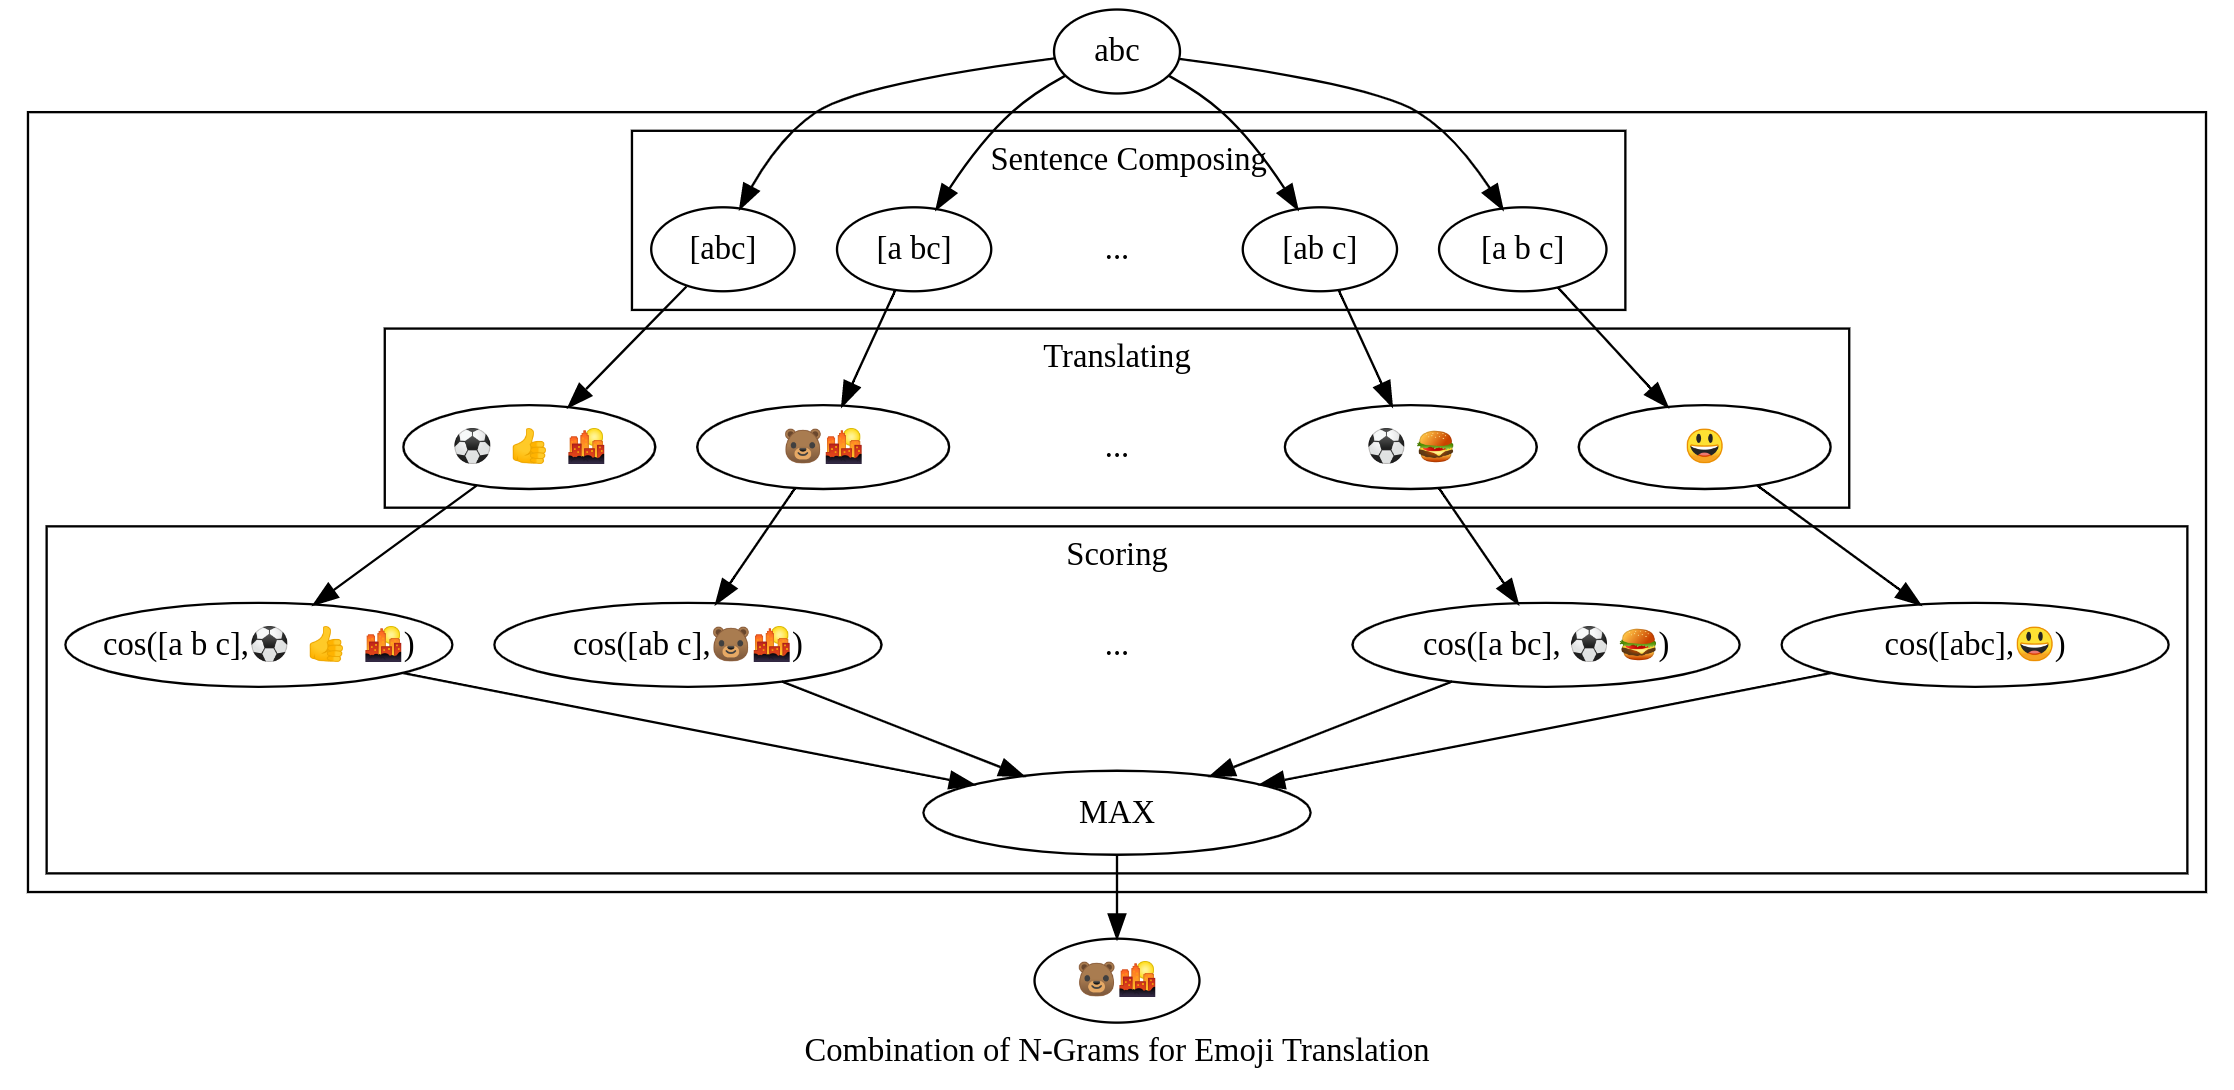
\includegraphics[width=0.90\textwidth]{figures/flow.png}
    \caption{The overall flow of the combination of N-grams in Emoji Translation
      (CoNFET) system\label{fig:flow}}
  \end{center}
\end{figure*}

\subsection{N-Gram Sequence Generation\label{sec:N-gramSequenceGeneration}}

The first part of the algorithm is splitting the sentence into a series
of n-grams denoted as an n-gram sequence. An n-gram is a selection of
words from a sentence. For example, the unigrams from the sentence ``The
dog bit me'' would be ``the'', ``dog'', ``bit'', and ``me''. Similarly,
the bigrams from that same sentence would be ``The dog'', ``dog bit'',
and ``bit me''. This sequence of n-grams would ideally split the
sentence into its constituent words and then translate them into emojis.
Two approaches have been applied for n-gram sequence generation.
Exhaustive generation, meaning that every n-gram sequence is generated
and tested is described in Section~\ref{sec:exhaustive}. The second approach, described
in Section~\ref{sec:dependency}, generates the sequence in a
way informed by the relations between words in the input sentence.

\subsubsection{Exhaustive N-Gram Sequence Generation\label{sec:exhaustive}}

The initial approach for the n-gram sequence generation was a brute
force approach that rests on the assumption that the optimal n-gram
sequence is made up of contiguous words within the input sentence. That
is, if the input is of the form ``a b c'', the optimal n-gram sequence
will never contain ``c a'', ``c b'', nor ``b a''. The optimal n-gram
sequence is defined as the sequence that produces the best summary.
These n-gram sequences are generated first by generating all
compositions of the integer that is equal to the length of the sentence.
Each of those compositions is then extrapolated into an n-gram sequence.
For example, the integer 3 can be generated by summing the elements in
the following arrays: [1, 1, 1], [1, 2], [2, 1], or [3].
Any one of those arrays can be turned into an n-gram sequence by taking
n-grams that are equal to the length of the element from the input
sentence. For example, [1, 1, 1] is translated into a sequence of 3
uni-grams. The major downside to this approach is computational
complexity. For a sentence with the word length~\(n\), this
algorithm generates~\(2^{n-1}\) sequences. While speed was not a
major concern with this algorithm, sentences with 10 or more words take
prohibitively long to translate.

Figure~\ref{fig:timing} depicts the translation time
for sentences with different lengths using the exhaustive and dependency
tree sentence composition algorithms. If the input sentence has more
than 10 words, the translation time using the exhaustive algorithm
increases exponentially. In fact, sentences with more than 11 words
results in a memory exception in the development environment when
trying to summarize with the exhaustive algorithm.

\begin{figure}[H]
  \begin{center}
    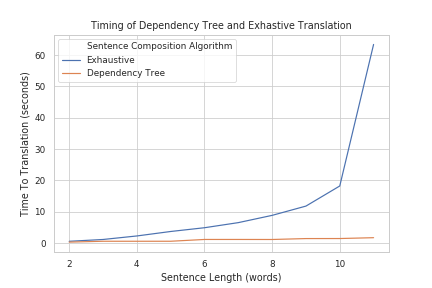
\includegraphics[width=\columnwidth]{figures/timing.png}
    \caption{Translation time of two n-gram sequence generation
      algorithms\label{fig:timing}}
  \end{center}
\end{figure}

\subsubsection{Dependency Tree Informed N-Gram Sequence Generation\label{sec:dependency}}

The second approach that was used to generate a representative n-gram
sequence is the dependency relations within a sentence.
Figure~\ref{fig:dep} shows an example of the sentence
``I finished my homework just before class started'' with the part of
speech tagging and the dependency relations. The dependencies can be
thought of as modifiers in the sense that the pronoun ``I'' modifies the
verb ``finished'' to inform who executed the action.

\begin{figure}[H]
  \begin{center}
    %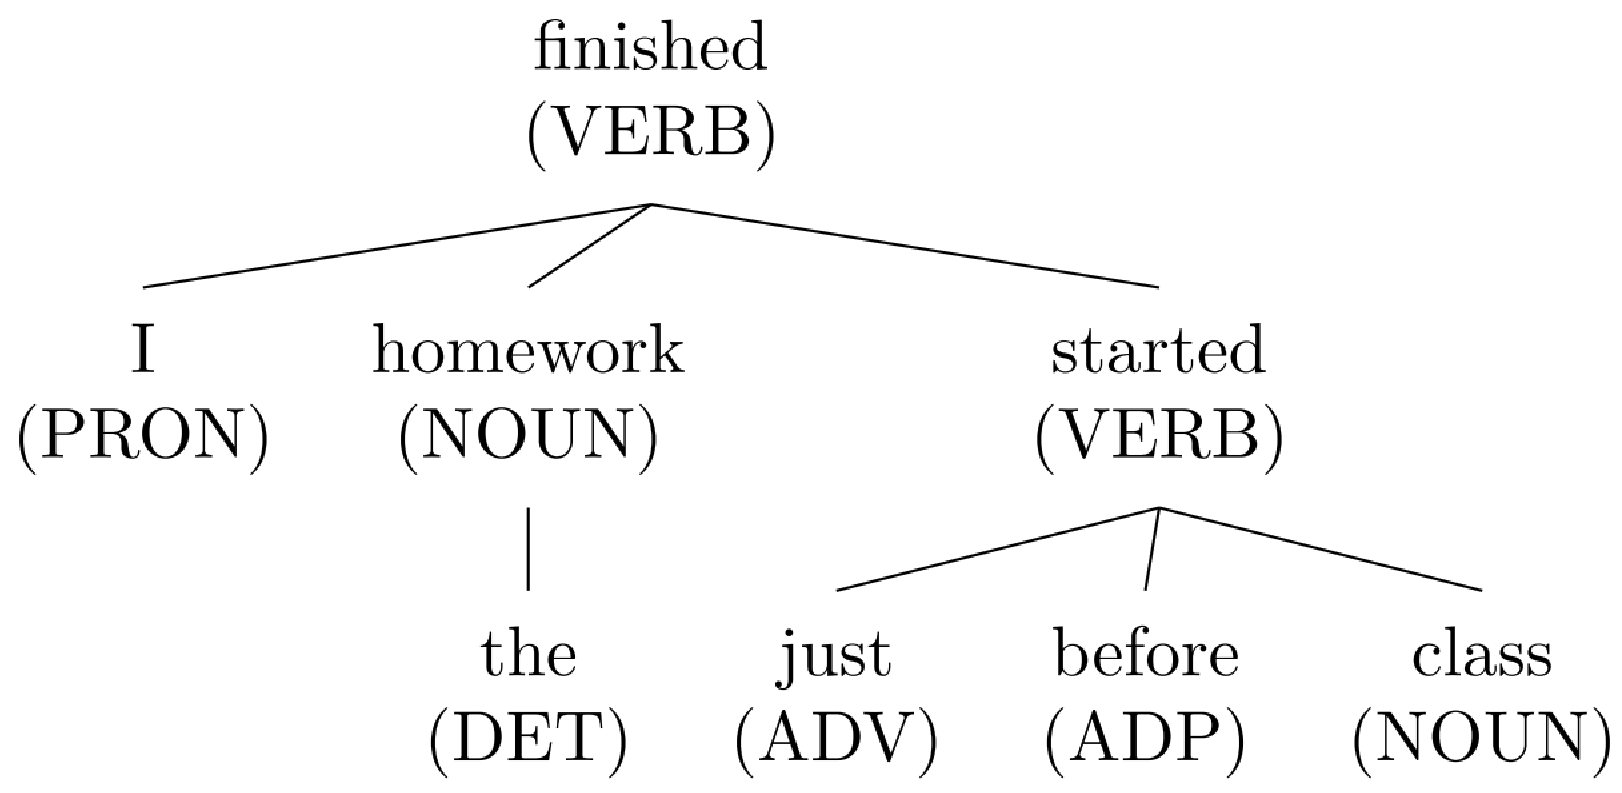
\includegraphics[width=0.90\columnwidth]{figures/syntax.png}
    \begin{forest}
      [finished\\(VERB)
        [I\\(PRON)]
        [homework\\(NOUN) [the\\(DET)]]
        [started\\(VERB)[just\\(ADV)][before\\(ADP)][class\\(NOUN)]]
      ]
    \end{forest}
    \caption{Dependency tree for ``I finished the homework just before class started''\label{fig:dep}}
  \end{center}
\end{figure}

This tree has certain redundancies that can be removed in order to form
larger groupings of words as nodes. There are two rules used for this
tree collapse:

\begin{enumerate}
    \item{If a parent has only one child, then these two words are combined}
    \item{If two or more leaves are on the same level with the same parents, then they are combined}
\end{enumerate}

An example of the first tree collapse rule, that is, the parent and
child relationship collapse, can be seen in
Figure~\ref{fig:childBefore} and Figure~\ref{fig:childAfter}. The nodes ``homework'' and
``the'' are highlighted in Figure~\ref{fig:childBefore} to
indicate that they fulfill the requirement of a parent with only one
child. These two nodes can be collapsed into one node as shown in
Figure~\ref{fig:childAfter}.

\begin{figure}[H]
  \begin{center}
    %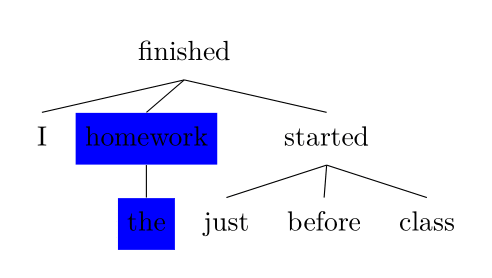
\includegraphics[width=0.90\columnwidth]{figures/child_before.png}
    \begin{forest}
      [finished
        [I]
        [homework, for tree={fill=cyan} [the]]
        [started[just][before][class]]
      ]
    \end{forest}
    \caption{Before the parent and child relationship tree collapse\label{fig:childBefore}}
  \end{center}
\end{figure}

\begin{figure}[H]
  \begin{center}
    %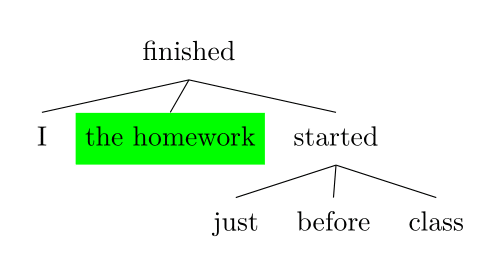
\includegraphics[width=0.90\columnwidth]{figures/child_after.png}
    \begin{forest}
      [finished
        [I]
        [the homework, for tree={fill=green}]
        [started[just][before][class]]
      ]
    \end{forest}
    \caption{After the parent and child relationship tree collapse\label{fig:childAfter}}
  \end{center}
\end{figure}

An example of the second tree collapse rule, that is, the leaf
relationship collapse, can be seen in
Figure~\ref{fig:beforeLeaf} and Figure~\ref{fig:afterLeaf}. In
Figure~\ref{fig:beforeLeaf}, the three leaf nodes ``just'',
``before'', and ``class'' are highlighted to indicate that they are the
only children of ``started'' and they are on the same level. These three
nodes can be collapsed into one node as shown in
Figure~\ref{fig:afterLeaf}.

\begin{figure}[H]
  \begin{center}
    % 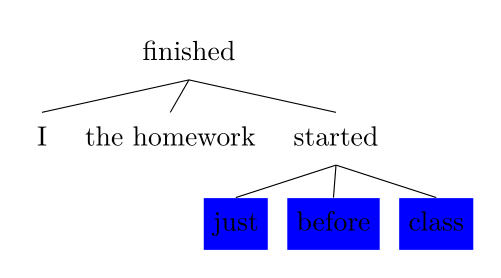
\includegraphics[width=0.90\columnwidth]{figures/leaf_before.png}
    \begin{forest}
      [finished
        [I]
        [the homework]
        [started[just, for tree={fill=cyan}][before, for tree={fill=cyan}][class, for tree={fill=cyan}]]
      ]
    \end{forest}
    \caption{Before the leaf relationship tree collapse\label{fig:beforeLeaf}}
  \end{center}
\end{figure}

\begin{figure}[H]
  \begin{center}
    % 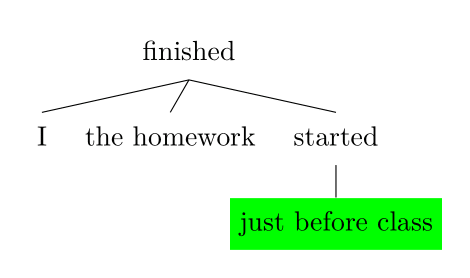
\includegraphics[width=0.90\columnwidth]{figures/leaf_after.png}
    \begin{forest}
    [finished
      [I]
      [the homework]
      [started[just before class, for tree={fill=green}]]
    ]
  \end{forest}
    \caption{After the leaf relationship tree collapse\label{fig:afterLeaf}}
  \end{center}
\end{figure}

\subsection{N-Gram to Emoji Translation\label{sec:n-gramToEmojiTranslation}}

The next step in the algorithm is to translate an n-gram sequence into
an emoji sequence. At its most basic, an emoji is purely a visualization
of a keyword. For example, the dog emoji (\img{emojis/1f415.png}) is a visual representation
of any of the following: ``dog'', ``puppy'', ``Shiba'', etc. With this
in mind, it is now simpler to find a way to draw comparisons between
n-grams and emojis. Both the emoji description and the n-gram in
question can be vectorized, so that a direct mathematical comparison can
be made. The vectorization is performed using
Sent2Vec~\cite{pg2017unsu}. Once the emoji and the n-gram are in the
same format, the cosine difference calculation is used for a direct
similarity comparison. The best emoji is defined as the emoji with a
description that has the lowest cosine difference to the n-gram.

\subsection{Translation Scoring\label{sec:translationScoring}}

Each n-gram sequence generated in
Section~\ref{sec:N-gramSequenceGeneration} is given a score based on the
individual n-gram cosine difference. Then, a sequence of the emojis
corresponding to the highest score becomes the output of the
summarization for the input sentence. Average cosine difference scoring
and weighing metric using the TF-IDF methods are used in our algorithm
and will be discussed in Section~\ref{sec:averageCosineDifference} and
Section~\ref{sec:TF-IDFWeighing}, respectively.

\subsubsection{Average Cosine Difference Scoring\label{sec:averageCosineDifference}}

A score for the overall n-gram sequence is generated by adding up the
cosine similarity of each n-gram composing the sequence and then
dividing by the number of n-grams as shown in Equation \refeq{eq:averageCosineDifference}.

\begin{equation}
   \textrm{Average Cos Difference Score} = \frac{\sum_{i=1}^{k}s_{i}}{k} \label{eq:averageCosineDifference}
\end{equation}

where~\(s_{i}\) is the cosine similarity for
the~\(i^{th}\) n-gram in the given n-gram sequence
and~\(k\) is the total number of n-grams within the n-gram
sequence.

\subsubsection{Weighing Metric using the TF-IDF\label{sec:TF-IDFWeighing}}

There are words that do not carry much semantic weight with
extraordinarily small cosine differences to certain emojis. For
instance, the word ``a'' maps directly to~~\img{emojis/1f4af.png}. In order to address the
varying impact of individual words, inspiration is drawn from one of the
abstractive summarization techniques, the Term Frequency- Inverse
Document Frequency (TF-IDF).

Using an open-source Python library Gensim~\cite{gensim}, the
TF-IDF scores are created for every term in a given corpus. It is
impractical to create n-grams of every possible length as the input
sentence could be any length; therefore, the document frequencies for
all n-grams except unigrams are estimated. To generate such a document
frequency for a given n-gram, two estimates are needed: the probability
that each term within the n-gram occurs together in a document and the
probability that the terms occur in the proper order. A naive estimate
of the chances of the constituent terms occurring in the same document
can be obtained by multiplying their document frequencies together as
shown in Equation \refeq{eq:TF-IDFWeighing}.

\begin{equation}
  P(a_{1} \land a_{2} \land \ldots \land a_{k} \in D) = \prod_{i=1}^{k}\textrm{DocFreq}(a_{i}, D) \label{eq:TF-IDFWeighing}
\end{equation}

where~\(a_{i}\) is the~\(i^{th}\) term in the n-gram,
~\(k\) is the total number of n-grams within the
n-gram sequence,~\(d\) is the document,
and~\(D\) is the corpus.

In order to obtain a similarly naive estimate of the terms occurring in
the necessary order, the input sentence is used as a template.
Considering the number of rearrangements of the words in the input
sentence with the terms in the n-gram in the proper order against all
possible rearrangements of the words gives the probability that the
n-gram appears in that sentence. Multiplying both of these values
together gives a weight for each individual n-gram within the sequence.
While there are issues with treating the words as independent (there
exist words like ``New'' and ``York'' that are frequently paired and in
some corpora occur together more often than either word independently)
and with treating a sentence as representative of a document, this
allows us to handle arbitrary n-grams as well as keep the dictionary a
manageable size. Now having a score for each n-gram within the sequence,
a score for that particular sequence can be obtained by weighing each
n-gram cosine similarity with its TF-IDF score and then averaging by the
TF-IDF score as shown in Equation \refeq{eq:averageTF-IDFScore}.

\begin{equation}
  \textrm{Average score weighted by
    TF-IDF} = \frac{\sum_{i=1}^{k}w_{i}\times s_i}{\sum_{i=1}^{k}w_{i}}\label{eq:averageTF-IDFScore}
\end{equation}

where~\(s_{i}\) is the cosine similarity score of
the~\(i^{th}\) n-gram and~\(w_{i}\) is the
corresponding TF-IDF weight.

The scores presented in the results section used the TF-IDF weighting
metric as it incoporated additional, meaningful analysis into the
score.

\subsection{Sentiment Emoji\label{sec:sentimentEmoji}}

One complication with the summarization process is that multiple phrases
map to the same emoji. With the few human translations considered, the
emotion behind the input sentence was not obvious after translated into
emojis. For example, both sentences ``Happy dog treats dog'' and ``Sad
dog treats dog'' map to~\img{emojis/1f415.png}\img{emojis/1f368.png}\img{emojis/1f415.png}. In an attempt to facilitate human
translation, a sentiment emoji was proposed. Tagging the sentence with a
\img{emojis/1f60a.png} or a \img{emojis/1f641.png} might allow humans to get closer to the input. Using the Python
library TextBlob~\cite{TextBlob}, a sentiment score is obtained for
the input sentence. It results in the polarity and subjectivity scores
that are corresponding to how positive and how factual TextBlob ranked
the input, respectively. Initially, the table~\cite{TextBlob} in
Figure~\ref{fig:sentimentTable} was used and the polarity is
ranged from -1 to 0 and the subjectivity is ranged from -1 to 1.

\begin{figure}[H]
  \begin{center}
    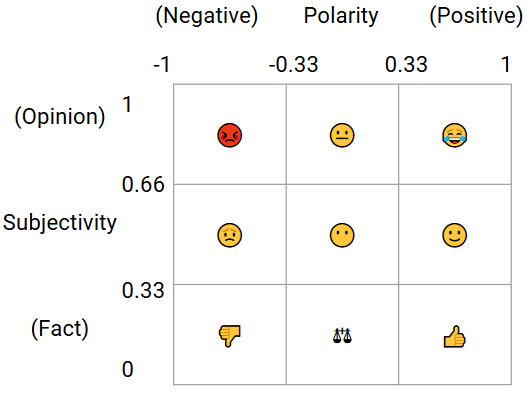
\includegraphics[width=0.90\columnwidth]{figures/sentiment_table1.png}
    \caption{Table used in conjunction with TextBlob for initial sentiment
      analysis\label{fig:sentimentTable}}
  \end{center}
\end{figure}

In order to allow more than the nine emojis seen in
Figure~{\ref{fig:sentimentTable}} to take the place of the
sentiment emoji as well as using emojis more in line with how they are
used on social media, an iteration was introduced. Using Twitter's
API, a number of tweets were gathered for each emoji. Each tweet was
scored using TextBlob and the scores for each emoji were averaged. Then,
the emoji with the sentiment score closest to the sentiment score of the
input sentence is selected as the sentiment emoji. The preliminary
results from scoring tweets are shown in Figure~\ref{fig:tweetScoring}. However, almost every
single emoji was clustered at zero. There are two reasons for this: the
size of the dataset and preprocessing of the tweet data. First, due to
Twitter's rate limit, the dataset gathered was fairly limited. The
issue is easily addressed by gathering data for a longer time. Secondly,
misspellings, slang, and grammatically incorrect sentences yield poor
results in TextBlob. For example, even a simple misspelling such as
``tightt'' for ``tight'' is enough to give the tweet a score of
zero. An implementation linking a dataset like Kaggle to sentiment
scores of the input sentence might yield more fruit.

\begin{figure*}[h]
  \begin{center}
    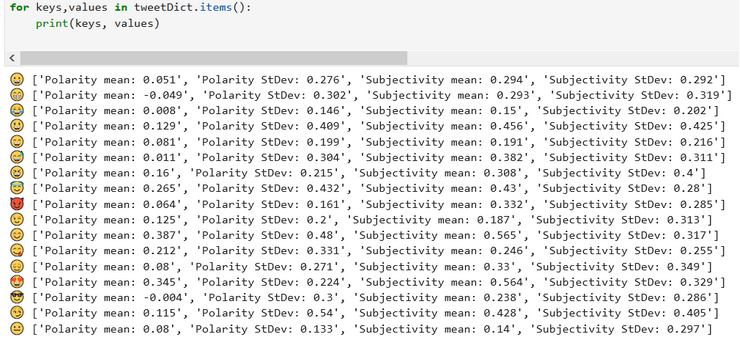
\includegraphics[width=0.90\textwidth]{figures/sentiment_results.png}
    \caption{Preliminary results from scoring tweets\label{fig:tweetScoring}}
  \end{center}
\end{figure*}


\section{Test Plan\label{sec:testPlan}}

Most translation algorithms are evaluated by comparing the output from
the algorithm to the known good translations. However, because there has
not been much work done in this English to emoji translation domain,
there was not a large enough sample data to test this algorithm on in
that fashion. Due to this fact, a new way to quantify the accuracy of
the translation algorithm was needed. The testing algorithm developed
starts by generating an emoji translation for a given number of input
sentences. These emoji translations are presented to a user for
translation back into English. A direct numerical comparison can then be
drawn between the input sentence to the algorithm and the sentence
provided by the human using the cosine difference between the vectorized
sentences. One major downside to this testing is that it is
human-in-the-loop, meaning that human interaction is needed to complete
the test. This leads to a slower overall testing process and removes the
ability to test at each iteration.~The general flow for this test
process is as follows:

\begin{enumerate}
\item
  Generate sentences in English.
\item
  Summarize each of the sentences using CoNFET.
\item
  Take the top 20 sentences sorted by the certainty score.
\item
  {For each machine translated sentence:}
    \begin{enumerate}
        \item
          {Provide the user with the emojis}
        \item
          {Provide the user with the length of the result sentence }
        \item
          {Prompt the user to translate the emojis into a sentence}
    \end{enumerate}
\item
  {For each pair of the machine translated sentence and the user
  translated sentence:}
    \begin{enumerate}
      \item
        {Calculate the distance between the two sentences using Sent2Vec}
    \end{enumerate}
\end{enumerate}

\section{Implementation\label{sec:implementation}}

All of the code for this project was written in Python 3, using the
following packages: SpaCy~\cite{spacy2}, NLTK~\cite{bird2009natural},
Gensim~\cite{gensim}, TextBlob~\cite{TextBlob},
~Sent2Vec~\cite{pg2017unsu}, NumPy\cite{numpy}, and
Jupyter\cite{Kluyver:2016aa}.

\section{Results\label{sec:results}}

The results from the exhaustive n-gram generation algorithm are
presented in Figure~\ref{fig:extractive}. Emojis are just
visualizations of specific descriptions as mentioned in Section 3.2. As
such, some of these translations may not make sense unless the specific
descriptions of emojis are known. For example, the n-gram ``They are
playing'' is translated to the emoji~\img{emojis/1f3b4.png} as shown in the third
test data in Figure~\ref{fig:extractive}. This emoji is known
as the ``Flower Playing Cards''. Once this description is known, the
emoji translated sentence makes more sense.

\begin{figure}[H]
  \begin{center}
    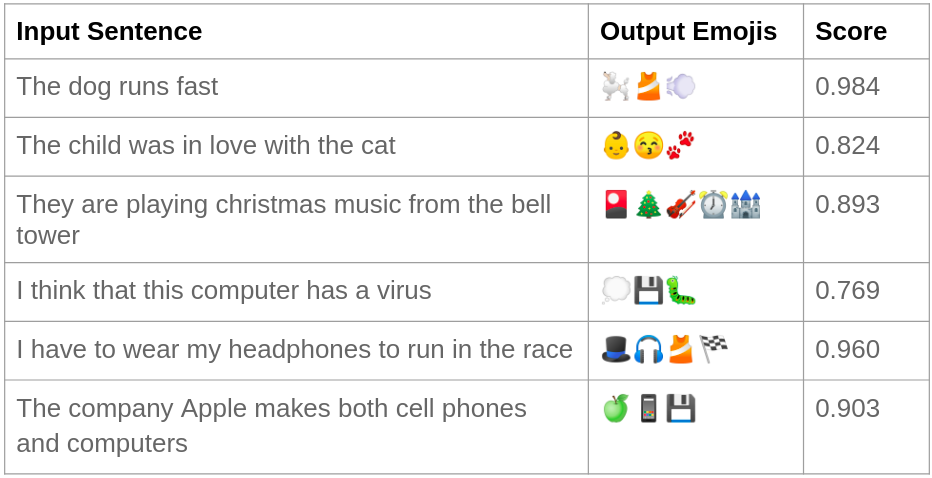
\includegraphics[width=0.70\columnwidth]{figures/extractive.png}
    \caption{Results from the exhaustive n-gram generation algorithm\label{fig:extractive}}
  \end{center}
\end{figure}

The results from the dependency tree n-gram generation algorithm are
presented in Figure~\ref{fig:dependency}. These summary
results are not as good as the results of the exhaustive algorithm.
This is mainly because the dependency tree algorithm does not take
into account the score that the translation of the proposed sequence
will have. On the other hand, the exhaustive algorithm splits the
sentence as to maximize the resulting score.
\begin{figure}[H]
  \begin{center}
    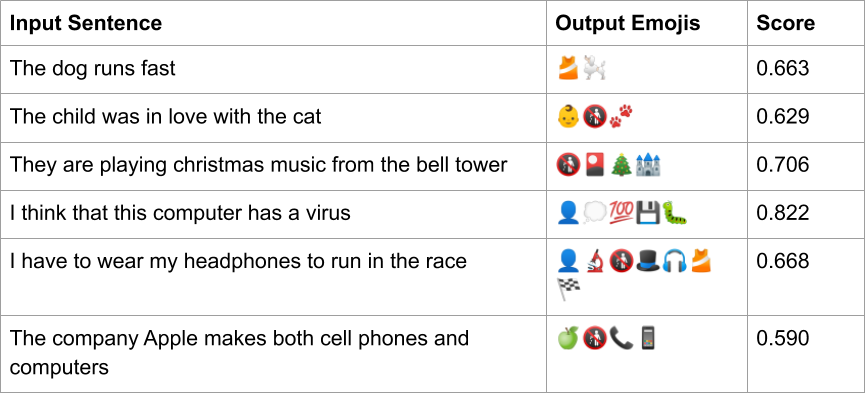
\includegraphics[width=0.70\columnwidth]{figures/dependency.png}
      \caption{Results from the dependency tree n-gram generation algorithm\label{fig:dependency}}
  \end{center}
\end{figure}

\section{Conclusion}

In this paper, a new algorithm for translation of English sentences
into a series of emojis, CoNFET is described. Emojis are becoming well
understood in the domain of Natural Language Processing, so they make
sense as an output medium for a new translation algorithm. CoNFET
accomplishes this goal through the use of the n-gram sequence generation
algorithms combined with the n-gram to emoji translation and the scoring
methods. This algorithm could be useful for the field of communication
between individuals with cognitive disabilities or for describing a long
document in a condensed way.

One of the main drawbacks of this implementation was the
limited dataset. The dataset defines the complexity of the output
language, it is used as a translation mapping from emojis to English
phrases and vice-versa. In the current implementation, there are 6,000
entries in the dataset and only 1662 unique emojis. In the future, some
exploration will be done with scraping different emoji database-like
sites (e.g. Emojipedia) to create a richer output language. In addition
to the size limitations, the dataset is also limited in the sense that
one keyword may have multiple emojis that represent it. In fact, in our
dataset, 15\%, around 720 descriptions have multiple emojis. This means
that some n-grams have multiple emojis that are all equally close. In
the future, we will investigate alternate heuristics by using the other
keywords of an emoji when deciding what translation is most suitable.
Finally, the last problem is that each n-gram is translated
individually. Therefore, no previous context in the sentence is be used
in the n-gram translation. If the previous n-grams can be taken into
account while translating the current n-gram, this may produce a more
representative emoji sequence. Also, the test plan detailed in
Section~\ref{sec:testPlan} should be implemented and
evaluated.

\makeatother
\bibliographystyle{PACISE}
\bibliography{biblio}

\end{document}
